\documentclass[border=10pt]{standalone}

\usepackage{tikz}
\usepackage{times}
\usetikzlibrary{arrows.meta, positioning, shapes.geometric, fit, calc}

\definecolor{frozen}{RGB}{200,200,220}
\definecolor{trainable}{RGB}{180,220,255}
\definecolor{comm}{RGB}{255,200,150}
\definecolor{envcolor}{RGB}{200,235,200}
\definecolor{losscolor}{RGB}{255,180,180}
\definecolor{gradcolor}{RGB}{220,50,50}

\begin{document}
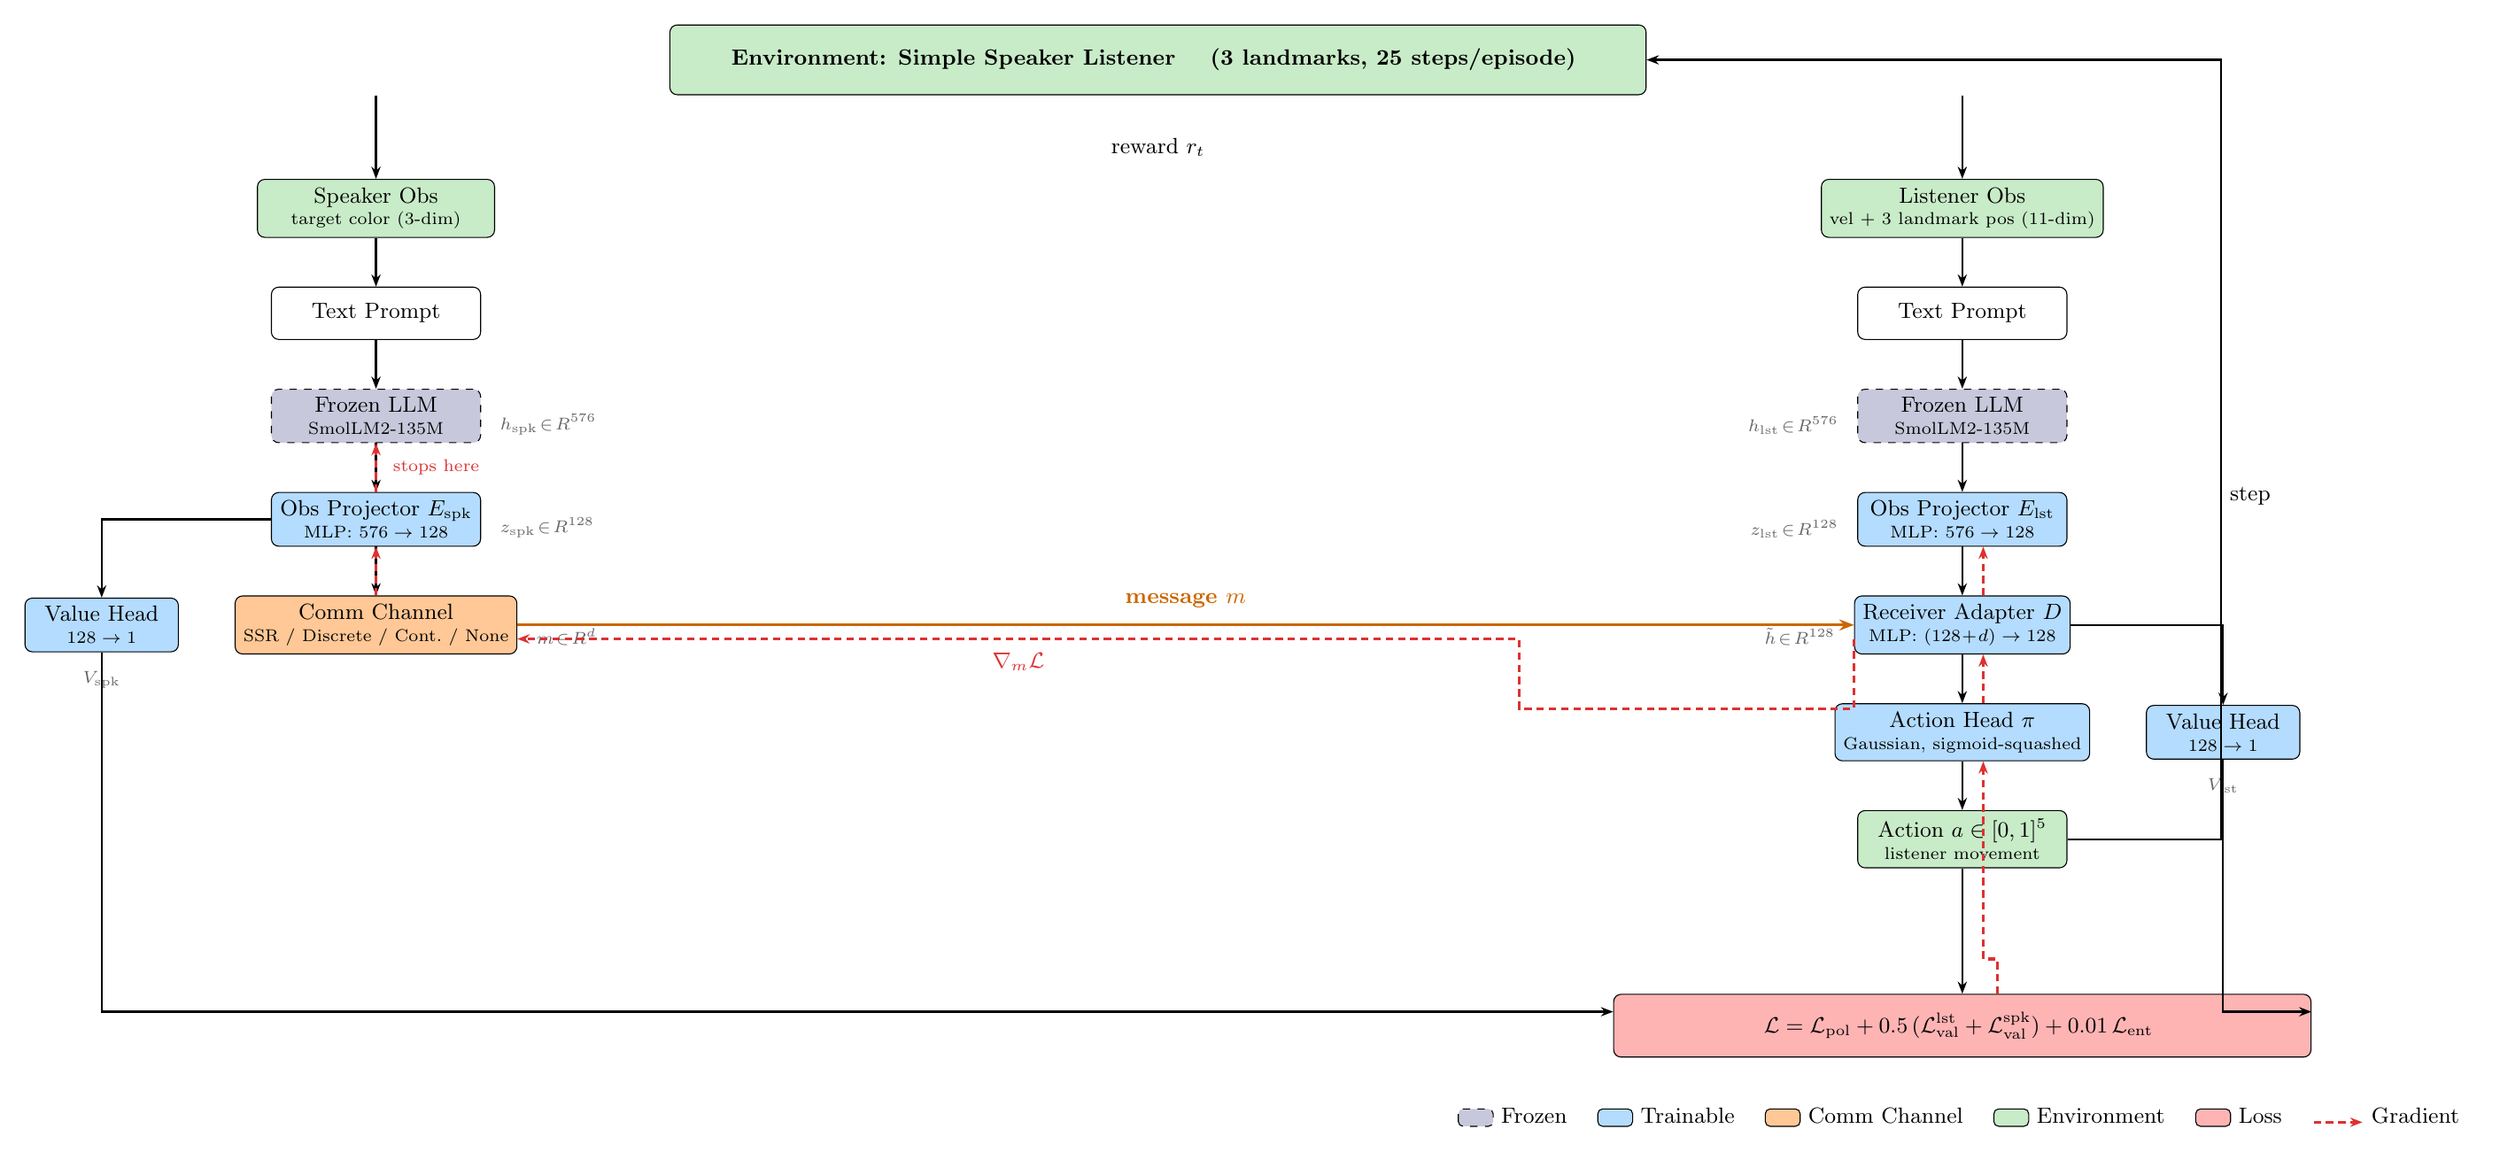
\begin{tikzpicture}[
    node distance=0.9cm and 2.5cm,
    box/.style={draw, rounded corners=3pt, minimum width=3cm, minimum height=0.75cm, align=center, font=\small},
    frozenbox/.style={box, fill=frozen, dashed},
    trainbox/.style={box, fill=trainable},
    commbox/.style={box, fill=comm, minimum width=3.2cm},
    envbox/.style={box, fill=envcolor},
    lossbox/.style={box, fill=losscolor},
    dataarrow/.style={-{Stealth[length=5pt]}, thick, black},
    gradarrow/.style={-{Stealth[length=5pt]}, line width=1.2pt, color=gradcolor, densely dashed},
    msgarrow/.style={-{Stealth[length=6pt]}, very thick, color=orange!80!black},
    dimlab/.style={font=\scriptsize, text=black!60},
    >={Stealth[length=5pt]},
]

% ===================== ENVIRONMENT =====================
\node[envbox, minimum width=14cm, minimum height=1cm, font=\small\bfseries] (env) {
    Environment: Simple Speaker Listener \quad (3 landmarks, 25 steps/episode)
};

% ===================== SPEAKER (left) =====================
\node[envbox, below left=1.2cm and 2.5cm of env, minimum width=3.4cm] (sobs) {
    Speaker Obs\\[-2pt]{\scriptsize target color (3-dim)}
};

\node[box, below=0.7cm of sobs] (sprompt) {Text Prompt};

\node[frozenbox, below=0.7cm of sprompt] (sllm) {
    Frozen LLM\\[-2pt]{\scriptsize SmolLM2-135M}
};

\node[trainbox, below=0.7cm of sllm] (sproj) {
    Obs Projector $E_{\mathrm{spk}}$\\[-2pt]{\scriptsize MLP: $576 \to 128$}
};

\node[commbox, below=0.7cm of sproj] (commch) {
    Comm Channel\\[-2pt]{\scriptsize SSR / Discrete / Cont.\ / None}
};

\node[trainbox, left=0.8cm of commch, minimum width=2.2cm] (vspk) {
    Value Head\\[-2pt]{\scriptsize $128 \to 1$}
};

% Dim labels speaker
\node[dimlab, right=0.15cm of sllm.south east, anchor=south west] {$h_{\mathrm{spk}} \!\in\! \mathbb{R}^{576}$};
\node[dimlab, right=0.15cm of sproj.south east, anchor=south west] {$z_{\mathrm{spk}} \!\in\! \mathbb{R}^{128}$};
\node[dimlab, right=0.15cm of commch.south east, anchor=south west] {$m \!\in\! \mathbb{R}^{d}$};
\node[dimlab, below=0.15cm of vspk] {$V_{\mathrm{spk}}$};

% ===================== LISTENER (right) =====================
\node[envbox, below right=1.2cm and 2.5cm of env, minimum width=3.4cm] (lobs) {
    Listener Obs\\[-2pt]{\scriptsize vel + 3 landmark pos (11-dim)}
};

\node[box, below=0.7cm of lobs] (lprompt) {Text Prompt};

\node[frozenbox, below=0.7cm of lprompt] (lllm) {
    Frozen LLM\\[-2pt]{\scriptsize SmolLM2-135M}
};

\node[trainbox, below=0.7cm of lllm] (lproj) {
    Obs Projector $E_{\mathrm{lst}}$\\[-2pt]{\scriptsize MLP: $576 \to 128$}
};

\node[trainbox, below=0.7cm of lproj] (adapter) {
    Receiver Adapter $D$\\[-2pt]{\scriptsize MLP: $(128\!+\!d) \to 128$}
};

\node[trainbox, below=0.7cm of adapter] (acthead) {
    Action Head $\pi$\\[-2pt]{\scriptsize Gaussian, sigmoid-squashed}
};

\node[trainbox, right=0.8cm of acthead, minimum width=2.2cm] (vlst) {
    Value Head\\[-2pt]{\scriptsize $128 \to 1$}
};

% Dim labels listener
\node[dimlab, left=0.15cm of lllm.south west, anchor=south east] {$h_{\mathrm{lst}} \!\in\! \mathbb{R}^{576}$};
\node[dimlab, left=0.15cm of lproj.south west, anchor=south east] {$z_{\mathrm{lst}} \!\in\! \mathbb{R}^{128}$};
\node[dimlab, left=0.15cm of adapter.south west, anchor=south east] {$\tilde{h} \!\in\! \mathbb{R}^{128}$};
\node[dimlab, below=0.15cm of vlst] {$V_{\mathrm{lst}}$};

% ===================== ACTION =====================
\node[envbox, below=0.7cm of acthead] (action) {
    Action $a \in [0,1]^5$\\[-2pt]{\scriptsize listener movement}
};

% ===================== LOSS =====================
\node[lossbox, below=1.8cm of action, minimum width=10cm, minimum height=0.9cm] (loss) {
    $\mathcal{L} = \mathcal{L}_{\mathrm{pol}} + 0.5\,(\mathcal{L}_{\mathrm{val}}^{\mathrm{lst}} + \mathcal{L}_{\mathrm{val}}^{\mathrm{spk}}) + 0.01\,\mathcal{L}_{\mathrm{ent}}$
};

% ===================== FORWARD ARROWS =====================
\draw[dataarrow] (env.south -| sobs) -- (sobs);
\draw[dataarrow] (sobs) -- (sprompt);
\draw[dataarrow] (sprompt) -- (sllm);
\draw[dataarrow] (sllm) -- (sproj);
\draw[dataarrow] (sproj) -- (commch);
\draw[dataarrow] (sproj.west) -| (vspk);

\draw[dataarrow] (env.south -| lobs) -- (lobs);
\draw[dataarrow] (lobs) -- (lprompt);
\draw[dataarrow] (lprompt) -- (lllm);
\draw[dataarrow] (lllm) -- (lproj);
\draw[dataarrow] (lproj) -- (adapter);
\draw[dataarrow] (adapter) -- (acthead);
\draw[dataarrow] (adapter.east) -| (vlst);
\draw[dataarrow] (acthead) -- (action);

% Message arrow
\draw[msgarrow]
    (commch.east) -- (adapter.west)
    node[midway, above=3pt, font=\small\bfseries, color=orange!80!black] {message $m$};

% Action back to env
\draw[dataarrow] (action.east) -- ++(2.2,0) |- (env.east)
    node[pos=0.22, right, font=\small] {step};

% Reward arrow
\node[below=0.5cm of env, font=\small] (reward) {reward $r_t$};

% Loss inputs
\draw[dataarrow] (action) -- (loss);
\draw[dataarrow] (vlst.south) |- ([yshift=2mm]loss.east);
\draw[dataarrow] (vspk.south) |- ([yshift=2mm]loss.west);

% ===================== GRADIENT ARROWS =====================
% From loss up through listener
\draw[gradarrow]
    ([xshift=5mm]loss.north) -- ++(0,0.5) -| ([xshift=3mm]acthead.south);

\draw[gradarrow]
    ([xshift=3mm]acthead.north) -- ([xshift=3mm]adapter.south);

\draw[gradarrow]
    ([xshift=3mm]adapter.north) -- ([xshift=3mm]lproj.south);

% Gradient through message back to speaker
\draw[gradarrow]
    ([yshift=-2mm]adapter.west) -- ++(0,0) -- ++(0,-1.0) -- ++(-4.8,0) -- ++(0,1.0) -- ([yshift=-2mm]commch.east)
    node[midway, below=2pt, font=\small\bfseries, color=gradcolor] {$\nabla_m \mathcal{L}$};

\draw[gradarrow]
    (commch.north) -- (sproj.south);

\draw[gradarrow]
    (sproj.north) -- (sllm.south)
    node[midway, right=3pt, font=\scriptsize, color=gradcolor] {stops here};

% ===================== LEGEND =====================
\node[below=0.6cm of loss, font=\small, align=center] {
    \tikz\draw[fill=frozen, draw, rounded corners=2pt, dashed] (0,0) rectangle (0.5,0.25); \raisebox{0.5mm}{Frozen} \quad
    \tikz\draw[fill=trainable, draw, rounded corners=2pt] (0,0) rectangle (0.5,0.25); \raisebox{0.5mm}{Trainable} \quad
    \tikz\draw[fill=comm, draw, rounded corners=2pt] (0,0) rectangle (0.5,0.25); \raisebox{0.5mm}{Comm Channel} \quad
    \tikz\draw[fill=envcolor, draw, rounded corners=2pt] (0,0) rectangle (0.5,0.25); \raisebox{0.5mm}{Environment} \quad
    \tikz\draw[fill=losscolor, draw, rounded corners=2pt] (0,0) rectangle (0.5,0.25); \raisebox{0.5mm}{Loss} \quad
    \tikz\draw[gradarrow] (0,0.12) -- (0.7,0.12); \raisebox{0.5mm}{Gradient}
};

\end{tikzpicture}
\end{document}
